\documentclass{beamer}
\usetheme{Madrid} % You can change this to your preferred theme

\setbeamercovered{transparent}


%references
\usepackage[backend=biber,style=authoryear]{biblatex} % or style=numeric
\addbibresource{MyLibrary.bib}
% square brackets for \cite (older biblatex compatibility)
\DeclareCiteCommand{\cite}[\mkbibbrackets]
  {\usebibmacro{prenote}}
  {\usebibmacro{citeindex}\usebibmacro{cite}}
  {\multicitedelim}
  {\usebibmacro{postnote}}



% Avoid block shadow artifacts (especially noticeable with pgfpages/notes layouts)
\setbeamertemplate{blocks}[rounded][shadow=false]

%for diagrams
\usepackage{tikz}
\usepackage{tikz-cd}
%for \mathrm
\usepackage{amsmath}
\DeclareMathOperator{\Det}{Det}
\DeclareMathOperator{\Tr}{Tr}

%for notes
\usepackage{pgfpages}
\setbeameroption{hide notes} % Only slides
 \setbeameroption{show notes on second screen=right} % <-- enable this only when you want notes
 \setbeamertemplate{note page}{\pagecolor{yellow!5}\insertnote} % optional note styling
\usepackage{palatino}

\title[Non-linear p-form gauge theories]{Non-linear p-form gauge theories and their deformations}
\subtitle{Master Degree in Physics --- Final Dissertation}
\author[Filippo Pesce]{%
  \texorpdfstring{Candidate: Filippo Pesce \\ \small Supervisors: Prof. Kurt Lechner, Prof. Dmitri Sorokin}{Candidate: Filippo Pesce; Supervisors: Prof. Kurt Lechner, Prof. Dmitri Sorokin}%
}
\institute[UniPD]{
  Dipartimento di Fisica e Astronomia ``Galileo Galilei'' \\
  Università degli Studi di Padova
}
\date{Academic Year 2025/2026}

\begin{document}

% The Title Slide
\begin{frame}
  \titlepage

    \note{Good morning to everyone, my thesis is entitled "Non-linear p-form gauge theories and their deformations".\newline
    This work was supervised by Professor Kurt Lechner and Professor Dmitri Sorokin.
    }
\end{frame}

%1st section------------------------------------------------
\section{Introduction}
%-----------------------------------------------------------

\subsection{Quantum Field Theories via ``deformations''}

\begin{frame}
    \frametitle{Studying QFTs via ``deformations''}

    Starting from a ``\textit{seed}'' theory described by a Lagrangian density $\mathcal{L}_0$, one way to deform the theory is to add an integrated local operator to the initial action

    \[\begin{aligned}
    S_0 &= \int d^d x \, \mathcal{L}_0(\phi,\partial_\mu\phi,...)\\[2pt]
    &\textcolor{blue}{\downarrow}\\
    S_\lambda &= S_0 + \lambda \int d^d x \, \mathcal{O}(\phi,\partial_\mu\phi,...) + o(\lambda^2).\\
    \end{aligned}\]

    \pause
    
    \begin{block}{Equivalent point of view: a flow (differential) equation}
    \[\begin{aligned}
    \frac{\partial S_\lambda}{\partial\lambda} &= \int d^d x\,\mathcal{O}^{(\lambda)}(\phi,\partial_\mu\phi,...)\,,
    \qquad S_{\lambda=0}=S_0.
    \end{aligned}\]
    \end{block}

    %\[
    %{\footnotesize \boxed{\;
    %\text{Free chiral }p\text{-form theory}
    %\;\xrightarrow{\;\text{stress-tensor deformations}\;}
    %\text{non-linear chiral }p\text{-form theory}}}
    %\]
    
    This thesis focuses on deformations of (chiral) $4$-form gauge theories in $d=10$, higher-rank analogues of Maxwell theory that arise naturally in string theory.

    \note{Let me start by introducing some general notions.\newline
    One powerful tool that we have to study quantum field theories is to begin with a simple, well-understood (``seed'') theory, that here is denoted with  $S_0$ and whose Lagrangian is function of some fundamental fields $\phi$ and their derivatives, and then deform it by adding an integrated local operator $\mathcal{O}$.\newline
    This operator will be multiplied for some constant parameter that we usually call $\lambda$ which measures how far we are from the original seed action: this defines a trajectory on the space of all QFTs that is parametrized by $\lambda$.\newline
    Equivalently, the same trajectory can be found by solving a differential equation, where the initial condition is that the seed action, which is usually a free theory like the Maxwell one, is recovered for $\lambda=0$.\newline
    In our thesis we have studied stress-tensor deformations of chiral 4-form theories, which are the higher-dimensional generalization of the Maxwell electrodynamics that appear naturally in String Theory. But what are stress-tensor deformations?}    
\end{frame}

\subsection{$\textrm{T}\bar{\textrm{T}}$-deformations}

\begin{frame}
    \frametitle{$\mathrm{T}\bar{\mathrm{T}}$-deformations}

    %Conformal theories are essentially scale invariant theories, relevant in many branches of physics.

    %\vspace{0.2cm}
    
    Rather surprisingly, the so called $\textrm{T}\bar{\textrm{T}}$-irrelevant deformation in $2d$ conformal field theories has gained much attention in the last decade

    \begin{block}{Zamolodchikov '04}
        \[\mathcal{O}^{(\lambda)}\equiv \Det(T_{\mu\nu}^{(\lambda)})=\textrm{T}\bar{\textrm{T}}^{(\lambda)}.\]
    \end{block}

    \begin{itemize}
        \item $T_{\mu\nu}^{(\lambda)}$ is the (deformed) stress-energy tensor.
    \end{itemize}
    
    What is special about $\rm{T}\bar{T}$-deformations?   

    \begin{itemize}[<+->]
        \item Universality;
        \item Solvability;
        \item Preserve many properties like supersymmetry and integrability.
    \end{itemize}

    \begin{block}<3->{Natural question}
        Can we extend this definition in $d>2$?
    \end{block}

    \note{Let me start from the beginning.\newline
    As we know conformal field theories, which are roughly speaking scale invariant theories, are important QFTs because they describe fixed points in RG theory and critical phenomena in statistical physics; in this setting, in particular in 2d CFT, Zamolodchikov introduced the so called "TTbar deformation". As we can see, this deformation is defined in terms of the determinant of the stress-energy tensor (of the deformed theory).\newline
    This particular deformation has very special properties.\newline
    First, it is universal, meaning it can be applied to a wide class of theories (basically any translational invariant 2d QFT).\newline
    Second, it is solvable, which means that many quantities of the
    deformed theory can be determined from the respective quantities
    of the undeformed one.\newline
    And third, it preserves important structures like integrability (which roughly speaking means that an infinite number of commuting charges remain conserved) and supersymmetry.\newline 
    Given these remarkable properties, people have wondered if this definition can be extended to higher dimensional settings.}

\end{frame}

\subsection{Non-linear electrodynamics}

\begin{frame}
\frametitle{Non-linear electrodynamics}

    Novel higher-dimensional realizations of stress-tensor deformations were discovered within non-linear electrodynamics (NED)

    %\begin{block}{NED action}
        %\[S_{\text{NED}}=\int d^4x\mathcal{L}(F_{\mu\nu}F^{\mu\nu},F_{\mu\nu}F^{\star\mu\nu})\]
    %\end{block}
    
    \[\boxed{S_{\text{NED}}=\int d^4x\mathcal{L}_{\text{NED}}(F_{\mu\nu}F^{\mu\nu},F_{\mu\nu}F^{\star\mu\nu})}\]
    {\footnotesize where $F^{\star}_{\mu\nu}\equiv \frac{1}{2}\,\varepsilon_{\mu\nu\rho\sigma}F^{\rho\sigma}$ is the Hodge-dual of the Maxwell tensor $F_{\mu\nu}$(in $d=4$).}

    \vspace{0.3cm}

    Important examples (both recover $\mathcal{L}_{\text{Max}}\equiv-\frac{1}{4}F_{\mu\nu}F^{\mu\nu}$ for $\gamma,\lambda\rightarrow0$):

    \begin{exampleblock}{ModMax theory, $\gamma\rightarrow$ dimensionless parameter}
    \[\mathcal{L}_{\text{ModMax}}^{(\gamma)}=-\frac{1}{4}\cosh(\gamma)F_{\mu\nu}F^{\mu\nu}
        +\frac{1}{4}\sinh(\gamma)\sqrt{(F_{\mu\nu}F^{\mu\nu})^2+(F^{\mu\nu}F^{\star}_{\mu\nu})^2},\]
    \end{exampleblock}

    \begin{exampleblock}{Born-Infeld theory, $\lambda\rightarrow$ dimensionful parameter}
    \[
    \mathcal{L}_{\text{BI}}^{(\lambda)}=\frac{\sqrt{-g}}{\lambda}-\frac{1}{\lambda}\sqrt{-\Det(g_{\mu\nu}+\sqrt{\lambda}F_{\mu\nu})}.
    \] 
    \end{exampleblock}

    %\begin{itemize}
        %\item Modified Maxwell theory (ModMax, $\gamma\rightarrow$ dimensionless parameter)
        %\[\boxed{\mathcal{L}_{\text{ModMax}}^{(\gamma)}=-\frac{1}{4}\cosh(\gamma)F_{\mu\nu}F^{\mu\nu}
        %+\frac{1}{4}\sinh(\gamma)\sqrt{(F_{\mu\nu}F^{\mu\nu})^2+(F^{\mu\nu}F^{\star}_{\mu\nu})^2},}\]
        %\item Born-Infeld theory (BI, $\lambda\rightarrow$ dimensionful parameter)
        %\[\boxed{\mathcal{L}_{\text{BI}}^{(\lambda)}=\frac{\sqrt{-g}}{\lambda}-\frac{1}{\lambda}\sqrt{-\Det(g_{\mu\nu}+\sqrt{\lambda}F_{\mu\nu})}.}\]
    %\end{itemize}


    \note{The answer is positive, in particular important progress has been made in the framework of non-linear electrodynamics.
    Non-linear extension of electrodynamic have been extensively studied as possible candidates for catching new physics. Their Lagrangian depends on the only two independent Lorentz invariant quantities that can be constructed from the Maxwell tensor $F_{\mu\nu}$  (we avoid derivatives of F to get rid of ghosts).\newline    
    Here I have put two important examples for our discussion (which both recover the free Maxwell theory when the deformation parameter is zero)
    \begin{itemize}
        \item The first one is the ModMax electrodynamic defined as the unique non-linear extension of Maxwell ED that preserve both conformal and duality invariance. It depends on a dimensionless parameter, while unitarity and causality bound the values of the parameter to be $\gamma\geq0$.
        \item The second one is instead the Born-Infeld theory which is duality invariant and appear in the String Theory context describing the worldvolume dynamics of  Dirichlet-branes. In this case the parameter $\lambda$ is dimensionful.
    \end{itemize}
    They can be both be obtained from dimensional reduction of six dimensional analogue theories.
    }
\end{frame}

\subsection{$\mathrm{T}\bar{\mathrm{T}}$ in $d=4$}

\begin{frame}
\frametitle{$\mathrm{T}\bar{\mathrm{T}}$ in $d=4$}

    ModMax and BI as $\textrm{T}\bar{\textrm{T}}$-like deformations of $4d$ Maxwell's theory

    \begin{center}
    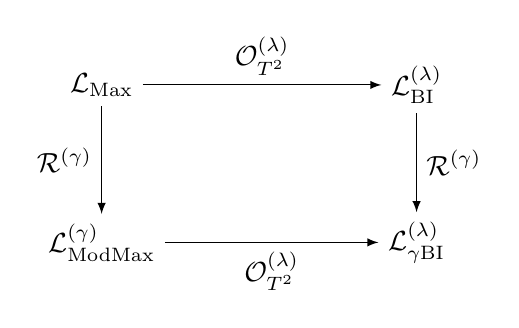
\begin{tikzpicture}[>=latex]
    \node (M) at (0,0) {$\mathcal{L}_{\mathrm{Max}}$};
    \node (BI) at (4,0) {$\mathcal{L}_{\mathrm{BI}}^{(\lambda)}$};
    \node (MM) at (0,-2) {$\mathcal{L}_{\mathrm{ModMax}}^{(\gamma)}$};
    \node (GBI) at (4,-2) {$\mathcal{L}_{\gamma\mathrm{BI}}^{(\lambda)}$};

    \draw[->] (M) -- node[above] {$\mathcal{O}_{T^2}^{(\lambda)}$} (BI);
    \draw[->] (M) -- node[left] {$\mathcal{R}^{(\gamma)}$} (MM);
    \draw[->] (MM) -- node[below] {$\mathcal{O}_{T^2}^{(\lambda)}$} (GBI);
    \draw[->] (BI) -- node[right] {$\mathcal{R}^{(\gamma)}$} (GBI);
    \end{tikzpicture}
    \end{center}

    where

    \begin{itemize}
        \item \resizebox{\linewidth}{!}{$\displaystyle
        \mathcal{O}^{(\lambda)}_{T^2}=\frac{1}{2d}\biggl(T^{(\lambda)\mu\nu}T^{(\lambda)}_{\mu\nu}-\frac{2}{d}(T^{(\lambda)\mu}_{\hspace{0.6cm}\mu})^2\biggr),\qquad
        \mathcal{R}^{(\gamma)}=\frac{1}{\sqrt{d}}\sqrt{T^{(\gamma)\mu\nu}T_{\mu\nu}^{(\gamma)}-\frac{1}{d}(T^{(\gamma)\mu}_{\hspace{0.5cm}\mu})^2}
        $;}
        \item \resizebox{\linewidth}{!}{$ \mathcal{L}_{\gamma\text{BI}}^{(\lambda)}\equiv\frac{1}{\lambda}\bigg\{1-\sqrt{1+\frac{\lambda}{2}\bigg[\cosh(\gamma)F^2-\sinh(\gamma)\sqrt{(F^2)^2+(FF^\star)^2}\bigg]-\frac{\lambda^2}{16}(FF^\star)^2}\bigg\}$.} 
    \end{itemize}


    \note{As mentioned before, surprising results regarding stress-tensor deformations have been obtained in this context: interestingly, if we deform the free Maxwell theory with this new marginal root-TTbar operator we get the Modified Maxwell Lagrangian. Instead deforming it with the $T^2$ operator gives the Born-Infeld theory. Moreover, if one deforms the BI theory with the root-TTbar operator ends up having a duality-symmetric generalization of the ModMax theory called "modified BI theory", whose weak field limit recovers the ModMax theory. 
    }
\end{frame}

%table of contents
\begin{frame}
\frametitle{Table of Contents}
\tableofcontents

\note{So far we introduced the definition of $\textrm{T}\bar{\textrm{T}}$-deformations and why they are so special.\newline 
In the second part, I will show what we have done to try to extend $\textrm{T}\bar{\textrm{T}}$-like deformations in ten dimensions, in particular in the context of chiral $4$-form theories in $d=10$. To do this I will have to first explain what chiral field theories are. We will then talk about some results regarding stress-tensor deformations in that setting. We will then specify our discussion to specific type of marginal deformations, the root-TTbar ones. To finish this second part of the discussion, we will show some details of our computation.\newline
In the conclusions I will give you our results and leave you some open questions that need further investigations.}
\end{frame}

%2nd section------------------------------------------------
\section{Can we extend $\textrm{T}\bar{\textrm{T}}$-like deformations to  $d=10$?}
%-----------------------------------------------------------

\subsection{Chiral $p$-form theories}

\begin{frame}
\frametitle{Chiral $p$-form theories}

    \begin{itemize}[<+->]
    \item Chiral $p$-form theories describe the dynamics of $p$-forms $A_{p}$ whose field strength $F_{p+1}=dA_p$ enjoys self-duality (in the linear theory)

    \[F^\star_{p+1}=F_{p+1};\]

    \item This condition is difficult to implement at the level of the action while preserving Lorentz invariance;
    \item The Ivanov-Nurmagambetov-Zupnik (INZ) approach solves this issue introducing, in the non-linear theory, an auxiliary field $\Lambda$

    \[\begin{aligned}
    \mathcal{L}_{\text{INZ}}^\gamma=\underset{\substack{\downarrow\\\text{\scriptsize PST}}}{\mathcal{L}_0}-\mathcal{V}(\Lambda,\gamma)\hspace{0.3cm}\text{where the e.o.m. are}\hspace{0.3cm}&\frac{1}{2}(F_{p+1}-F^\star_{p+1})=\frac{\partial\mathcal{V}}{\partial\Lambda},\\
    &\Lambda=-\frac{1}{2}(F_{p+1}+F^{\star}_{p+1});
    \end{aligned}\]

    %\resizebox{\linewidth}{!}{$F^-_{p+1}=\frac{1}{2}(F_{p+1}-F^\star_{p+1})=(p+1)\frac{\partial\mathcal{V}}{\partial\Lambda}$,\hspace{0.3cm}$\Lambda_{p+1}=-\frac{1}{2}(F_{p+1}+F^{\star}_{p+1})$};

    \item We studied whether this class of non-linear Lagrangians can be viewed as stress tensor deformations of the free Lagrangian $\mathcal{L}_0$. 
    
    \end{itemize}

    \note{As anticipated, some interesting results have been obtained also in the context of chiral field theories. So let me summarize what chiral $p$-form theories are.\newline
    In these theories the fundamental objects are $p$-forms whose exterior derivative defines the so called "field strength". The main feature of chiral field theory is that this field strength enjoys self-duality condition in a manifest way (as solution of the EOM of $A_p$).
    Unfortunately, this duality condition is difficult to implement at the level of the action while keeping Lorentz invariance. For this reason, the Ivanov-Nurmagambetov-Zupnik approach comes to rescue by introducing an auxiliary  field $\Lambda$. 
    This INZ framework allows us to write a consistent covariant action and makes it suitable for studying deformations.  The INZ Lagrangian contains a kinetic term (which gives the linear self-duality condition above) plus some potential $\cal{V}$ accounting for self-interactions. As we can see, in this formulation the anti-self dual part of the field strength is proportional to the derivative of $\cal{V}$ with respect to $\Lambda$ (so is zero for the free theory). Instead the auxiliary field turns out to be minus the self dual part of $F$, so if plugged in this first relation gives a non-linear self-duality condition which generalize this first one. In our work we have studied whether this class of non-linear Lagrangians can be viewed as stress-tensor def. of free chiral theories $L_0$.}
\end{frame}

%\subsection{Deformations of chiral $p$-form theories}

%\begin{frame}
%\frametitle{Deformations of chiral $p$-form theories}

    
    %Once we deform the INZ theory we introduce a dependence on the deformation parameter $\gamma$

    %\vspace{0.3cm}

    %\begin{block}{Deformed INZ Lagrangian}
    %\[
    %\boxed{
    %\mathcal{L}^{(\gamma)}_{\mathrm{INZ}}
    %=
    %\mathcal{L}_0
    %-\frac{1}{p!}\,\mathcal{V}(\Lambda,\gamma)
    %}
    %\]
    %\end{block}

    %\vspace{0.2cm}

    %where

    %\begin{itemize}
        %\item $\mathcal{L}_0$ is the free chiral %$p$-form Lagrangian;
        %\item $\Lambda$ is the auxiliary field introduced by the INZ formulation;
        %\item $\mathcal{V}(\Lambda,\gamma)$ is a relativistic invariant function of components of the auxiliary field $\Lambda$.
    %\end{itemize}

    %\vspace{0.2cm}

    %\note{These chiral theories can then be deformed, in particular the deformed Lagrangian will be like this: there is the free kinetic term and the self-interacting potential, which will depend on the deformation parameter now. This function is dependent on all the possible independent Lorentz invariants that one can build out of $\Lambda$. \newline
    %}
    
%\end{frame}

\subsection{$\mathrm{T}\bar{\mathrm{T}}$-flow in higher dimensions}

\begin{frame}[fragile]
\frametitle{$\mathrm{T}\bar{\mathrm{T}}$-flow in higher dimensions}

    
    
    In $d=4,6$ all non-linear electrodynamics and all chiral $2$-form theories are solutions of 
        \[\partial_\gamma\mathcal{L}^{(\gamma)}=f(T_{\mu\nu}^{(\gamma)},\gamma),\]
        $\mathcal{L}|_{\gamma=0}$ being the free (Maxwell or chiral $2$-form) theory.

    \begin{alertblock}{This classification is no longer true in $d=10$ [Lechner, Sorokin, Hutomo '25]}
    \small
    There are additional independent invariants (not expressible solely in terms of the stress-energy tensor) that obstruct writing a universal $\mathrm{T}\bar{\mathrm{T}}$-like flow.
    \end{alertblock}

    \pause

    \[\color{blue}{\downarrow}\]

    \begin{block}{Natural question addressed in this thesis}
    Can we find a subclass of chiral $4$-form theories in $d=10$ that obeys the $\rm{T}\bar{\rm{T}}$-like flow equation?
    \end{block}

    \note{A central result concerning stress-tensor deformations of chiral gauge field theories has been discovered in the last few years. That is, in dimensions 4 and 6 (in 2 dimensions the root TTbar flow has been shown to bring the theory of N free scalar bosons into the dimensional reduced ModMax theory), all non-linear duality-invariant theories of ED in $4d$ and all chiral $2$-form theories in $6d$ can be obtained as solutions of T-bar-T-like flow equations. This means that they are solution of a flow equation like the following one, where the initial condition is either the free Maxwell or the free chiral theory. \newline
    Unfortunately, in a recent work it has been shown with a counterexample that this beautiful property doesn't extend to $d=10$. The reason is that in $d=10$ there are too many Lorentz invariants, some of which can not be written in terms of the stress-energy tensor. Hence a natural question that we addressed in this thesis is:- Can we still find a subclass of chiral 4-form theories obeying such a flow equation?}
\end{frame}

\subsection{Root-$\textrm{T}\bar{\textrm{T}}$ flow in $d=10$}

\begin{frame}
\frametitle{Root-$\textrm{T}\bar{\textrm{T}}$ flow in $d=10$}
    We have focused on the flow equation

    \[
    -\partial_\gamma\mathcal{V} =\frac{1}{\sqrt{d}}\sqrt{T^{(\gamma)\mu\nu}T_{\mu\nu}^{(\gamma)}-\frac{1}{d}(T^{(\gamma)\mu}_{\hspace{0.5cm}\mu})^2}= \mathcal{R}^{(\gamma)}
    \]

    \vspace{0.3cm}

    \begin{itemize}[<+->]
    \item Universal for ModMax theories in $d=2,4,6$
    \[\mathcal{V}_{\text{ModMax}}^{\text{6d}}(\gamma,\Lambda)=-\frac{1}{2\sqrt{6}}\tanh(\frac{\gamma}{2})\sqrt{\Lambda^4};\]
    \item Exact solution unknown in $d=10$.
    \end{itemize}

    \vspace{0.3cm}
    
    \begin{block}<3->{Our approach in $d=10$}
    \[\text{Working perturbatively in $\gamma$}\]
    \end{block}

    \note{To address this problem, given the recent advancements we decided to focus on the specific flow equation involving the root-TTbar operator introduced in the first slides.
    The solution is known in lower dimensions, for example here I have put the 6d solution which contains an hyperbolic tangent of $\gamma$ multiplying the unique functionally independent Lorentz invariant quantity that you can build out of $\Lambda$. On the other hand no exact solution is known in 10 dimensions.\newline
    In short what we did was solving this equation order by order in the deformation parameter.
    We expanded the Lagrangian in powers of the deformation parameter gamma and computed $\mathcal{R}^{(\gamma)}$ order by order, starting from the free theory.
    }
    
\end{frame}

\subsection{Some details of the computation}
%-----------------------------------------------------------
% Optional “heavy computation” slide (edit with your actual result)
\begin{frame}[fragile]
\frametitle{Some details of the computation}

\begin{itemize}
\item $I_4\equiv \frac{1}{(2\cdot4!)^2}T^{(0)}_{\mu\nu}T^{(0)\mu\nu}\hspace{0.5cm}\text{with}\hspace{0.5cm} \Lambda_{\mu\alpha(4)}\Lambda_{\nu}^{\hspace{0.2cm}\alpha(4)}=\frac{1}{2\cdot4!}T_{\mu\nu}^{(0)}\equiv M_{\mu\nu}$;
\end{itemize}

\vspace{0.2cm}
\scriptsize
\begin{block}{Third order expansion}
\begin{align*}
    \mathcal{R}^{(1)}=&\frac{1}{\sqrt{10}}\sqrt{\frac{I_4}{(2\cdot 4!)^2}}\\
    \mathcal{R}^{(2)}=&-\frac{5}{2\cdot(4!)^3\sqrt{40}\sqrt{I^3_4}}M^{\mu}_{\hspace{0.2cm}\nu}M^{\hspace{0.2cm}\alpha}_{[\rho_1}\Lambda_{\rho_2\rho_3\rho_4\mu]\alpha}M^{[\rho_1}_{\hspace{0.2cm}\widetilde\alpha}\Lambda^{\rho_2\rho_3\rho_4\nu]\widetilde\alpha}\\
    \mathcal{L}'''_\gamma=&\mathcal{L}'_\gamma+\frac{\gamma^3}{3}\mathcal{R}^{(2)}\\
    =&\mathcal{L}_0+\frac{\gamma}{\sqrt{10}}\sqrt{\frac{I_4}{(2\cdot 4!)^2}}-\frac{5\gamma^3}{6(4!)^3\sqrt{40I^3_4}}M^{\mu}_{\hspace{0.2cm}\nu}M^{\hspace{0.2cm}\alpha}_{[\rho_1}\Lambda_{\rho_2\rho_3\rho_4\mu]\alpha}M^{[\rho_1}_{\hspace{0.2cm}\widetilde\alpha}\Lambda^{\rho_2\rho_3\rho_4\nu]\widetilde\alpha}.
\end{align*}
\end{block}

\vspace{0.1cm}
%\tiny
%\textit{(Optional) Report: number of terms after simplification, runtime, and independent cross-checks (e.g., self-duality + EOM consistency).}

\note{Just to give some taste of what we did, here I have shown the third order Lagrangian that we obtained using the perturbative approach. This $I_4$ is the unique independent fourth order invariant that one can build out of $\Lambda$, and is defined in terms of a symmetric matrix $M_{\mu\nu}$ built from $\Lambda$ itself and which coincides with the stress-energy tensor computed by means of the seed theory $\cal{L}_{0}$.\newline
The invariant combination that appear in the third order term is present also in the solution of the $T^2$-flow. This is not the final result since, in order to compare this solution to the six dimensional one, we had to elaborate on this combination to see how many terms inside it were $\propto \sqrt{I_4}$.
}
\end{frame}

%3rd section------------------------------------------------
\section{Conclusions}
%-----------------------------------------------------------

\subsection{Perturbative result}

\begin{frame}{}
\frametitle{Perturbative result}
    In six dimensions \textcolor{blue}{\cite{ferkoInteractingChiralForm2024}}
    
    \[\mathcal{L}^{(\gamma)}_{6d}=\mathcal{L}_0+\frac{1}{2\sqrt{6}}\tanh(\frac{\gamma}{2})\sqrt{I_4}.\]
    
    In ten dimensions instead we obtained

    \begin{alertblock}{}
    \[
    \mathcal{L}_{\gamma}^{'''}=\mathcal{L}_0+\frac{\sqrt{I_4}}{\sqrt{10}}\bigg(\frac{\gamma}{48}-\frac{1}{70}\frac{\gamma^3}{(4!)^3}\bigg)+\frac{1}{42\sqrt{40}}\frac{I_8}{I_4^{3/2}}\frac{\gamma^3}{(4!)^3}+\cdots,
    \]
    \[\text{where}\hspace{0.5cm}I_4\equiv \Tr(M^2),\hspace{0.5cm}I_8\equiv \Tr(M^4).\]
    \end{alertblock}

    \vspace{0.3cm}

    \vspace{0.3cm}

    \begin{alertblock}{The result}
    In comparison with the 6d chiral 2-form theory case, in 10d we found that already at $\gamma^3$ new invariant structures start to appear in the deformed action.
    \end{alertblock} 

    \note{Indeed as we already said, in six dimensions the flow equation has a well known solution given by the hyperbolic tangent of the deformation parameter times the square root of the unique fourth order Lorentz invariant that one can build out of the auxiliary field $\Lambda$. This is essentially the ModMax theory in $6d$.
    In ten dimensions there are many more independent invariants that one can build, and what we find is that the Lagrangian admits an expansion in odd powers of gamma: first order, third order, and so on.
    We also found that already at the third order in the expansion appear higher order invariants, differently from what happens in $6d$. Moreover the $\sqrt{I_4}$-branch does not show evidence of resumming into the hyperbolic form familiar from the $6d$ case.}    
\end{frame}

\subsection{Future directions}

\begin{frame}
\frametitle{Future directions}
    Several directions remain open:\newline

    \begin{itemize}[<+->]
        \item Extend the expansion to the next order;  
        %\item Explore the solution of $\textrm{T}\bar{\textrm{T}}$-like flows via dimensional uplift;
        \item Study possible supersymmetric generalizations of non-linear chiral $p$-form theories with the focus on String Theory applications;
        \item Study the fundamental origin of ModMax;       
        
    \end{itemize}

    \note{I'd like to conclude by mentioning a few possible future directions. One thing that would be interesting to sudy is the next order of the expansion, which requires advanced software calculus like Mathematica. This would provide a definitive proof that the 10d and 6d solutions deviate.
    Next, it would be intriguing to study new supersymmetric generalizations of chiral p-form theories and see how supersymmetry constraint the action: in particular it would be interesting to see how SUSY constraint how the self-dual five form enter the $d=10$ type IIB supergravity effective action. Another open problem is to explore the fundamental origin of ModMax: non linear ED must be considered as effective theories, so one may wonder whether it arise in some conformal limit of a Maxwell theory coupled to an axion-like field.}    
\end{frame}

\begin{frame}
\begin{center}
\huge{Thank you for the attention!}
\end{center}    
\end{frame}

\note{Thank you for the attention. I'll be happy to take questions.}

% --- Backup slide(s) for Q\&A ---

\begin{frame}
\frametitle{Specialness of $\mathrm{T}\bar{\mathrm{T}}$-deformations}

    The $\mathrm{T}\bar{\mathrm{T}}$ in $2d$ enjoys many important properties:

    \begin{enumerate}[<+->]
    \item \textbf{Factorization}: Zamolodchikov has shown that the expectation values factorize
    \[\langle\mathrm{T}\bar{\mathrm{T}}\rangle=\langle T\rangle\langle \bar{T}\rangle-\langle \Theta\rangle^2;\]
    \item \textbf{Finite volume spectrum}: the cylinder energy levels of a $\mathrm{T}\bar{\mathrm{T}}$-deformed theory obey a partial differential equation
    \[\partial_{\lambda}\mathcal{E}_{n}(R,\lambda)=\mathcal{E}_n(R,\lambda)\partial_{R}\mathcal{E}_{n}(R,\lambda)+\frac{1}{R}P_{n}(R)^{2};\]
    \item \textbf{Stringy behavior}: the $\textrm{T}\bar{\textrm{T}}$-deformation of a free boson in $2d$ results in the Gauge-fixed Nambu-Goto Lagrangian.
\end{enumerate}
    \note{Let me highlight a few key properties that make T-bar-T so special. \newline
    First, there is a remarkable factorization property discovered by Zamolodchikov: the expectation value of the $T\bar{T}$ operator factorizes into expectation values of the energy-momentum tensor itself: here $\Theta$ is just the trace of $T_{\mu\nu}$. \newline
    Second, using the previous property one can show that the energy levels in some cases satisfy a non-linear differential equation, which can actually be solved to obtain the deformed energy spectrum in terms of the undeformed ones. Here for example we are considering a $2d$ CFT defined on a cylinder. \newline
    Third, and maybe most strikingly, applying this deformation to a free boson leads to the Nambu–Goto action that appears in string theory. \newline
    So, in a sense, this flow connects simple field theories to objects that resemble string dynamics. \newline
    That’s already a hint that something deep is going on.}
\end{frame}

\begin{frame}
\frametitle{Specialness of $\mathrm{T}\bar{\mathrm{T}}$-deformations}

\begin{enumerate}[<+->]
\setcounter{enumi}{3}
    \item \textbf{Exact solvability}: several observables remain computable along the flow:
    \begin{itemize}
        \item torus partition function;
        \item under $\textrm{T}\bar{\textrm{T}}$ deformation the S matrix of a scattering process in $1+1$ dimensions gets a \textit{dressing factor}
        \[S(\{p_i\})\longrightarrow\bigg(\prod_{i<j }e^{-i\delta_{ij}^{(\lambda)}}\bigg)S(\{p_i\});\]
    \end{itemize}

\vspace{0.3cm}

    \item \textbf{Connections with gravity and holography}: $\mathrm{T}\bar{\mathrm{T}}$ deformations are related to:
    \begin{itemize}
        \item two-dimensional gravity;
        \item finite-cutoff AdS holography.
    \end{itemize}

\end{enumerate}

\note{Another interesting property of the TTbar deformation is that, in 1+1 dimensions, the deformed S matrix of a scattering process is equal to the initial one dressed with a CDD factor. This also implies that the TTbar deformation preserve integrability.\newline
Other observables can be computed from the undeformed ones, like the finite volume spectrum and the torus partition function.\newline
Also, it has been shown that turning on TTbar deformation for a QFT is equivalent to coupling the theory to a specific 2d topological gravity which is very similar to the JT gravity.\newline
Last but not least it has been argued that, for pure gravity, TTbar deformation corresponds to putting a Dirichlet boundary condition at finite radius in the bulk. This means that $\textrm{T}\bar{\textrm{T}}$ is equivalent to take the spacetime and cut it at finite radius.
}

\end{frame}

\begin{frame}
\frametitle{The explicit form of the INZ Lagrangian}

    \small
    A convenient explicit form is the action

    \[\begin{aligned}
    S_{\text{INZ}}[A,\Lambda,v]
    &\equiv \frac{1}{p!}\int d^{d}x\,\sqrt{-g}\;\mathcal{L}_{\text{INZ}},\\[2pt]
    \mathcal{L}_{\text{INZ}}
    &=\frac{1}{2}\,E\cdot B-\frac{1}{2}\,B\cdot B+(B+\lambda)\cdot(B+\lambda)
      -\mathcal{V}(\Lambda,g),
    \end{aligned}\]

    with the shorthand
    \begin{itemize}
        \item $F=dA$, \; $F^{\star}=\star F$, \; $v^2=-1$, \; $v_{\mu}(x)=\frac{\partial_{\mu}a(x)}{\sqrt{-(\partial_{\nu}a\partial^{\nu}a})}$;
        \item $E_{\mu_1\dots\mu_p}\equiv F_{\mu_1\dots\mu_p\nu}\,v^{\nu}$, \; $B_{\mu_1\dots\mu_p}\equiv F^{\star}_{\mu_1\dots\mu_p\nu}\,v^{\nu}$;
        \item $\lambda_{\mu_1\dots\mu_p}\equiv \Lambda_{\mu_1\dots\mu_p\nu}\,v^{\nu}$, \; $X\cdot Y\equiv \frac{1}{p!}X_{\mu_1\dots\mu_p}Y^{\mu_1\dots\mu_p}$.
    \end{itemize}

    \note{In this slide I have put the explicit form of the INZ Lagrangian. As we can see, here the generalized electric and magnetic fields are given by contracting the field strength to this new vector field $v^\mu$, which is not a physical field but rather a gauge d.o.f.}
\end{frame}

\begin{frame}
\frametitle{Gauge symmetries of the INZ Lagrangian}

    The INZ Lagrangian is invariant under the following gauge symmetries:

    \vspace{0.2cm}

    \begin{itemize}
        \item Setting $\mathfrak{E}_{\mu(p)}\equiv E_{\mu(p)}-B_{\mu(p)}$ the first one is
        \[\delta A_{\mu(p)}=\frac{\varphi}{\sqrt{-(\partial a)^2}}[\mathfrak{E}+2(B+\lambda)]_{\mu(p)},\hspace{0.5cm}\delta a=\varphi,\hspace{0.5cm}\delta\Lambda_{\mu(p+1)}=0,\]
        \item The second one is 
        \[\delta A_{\mu(p)}=v_{[\mu_1}\psi_{\mu_2...\mu_p]},\hspace{1cm}\delta a=0,\hspace{1cm}\delta\Lambda_{\mu(p+1)}=0.\]
    \end{itemize}

    \note{These gauge symmetries are necessary for a consistent description of chiral fields. In both cases the auxiliary field is left unchanged. The field $a(x)$ can be shown to be a pure gauge d.o.f.}
    
\end{frame}

\begin{frame}
\frametitle{Conformal invariant chiral $p$-form theories}

    \begin{itemize}[<+->]
        \item The stress-energy tensor of the INZ Lagrangian takes the form
        \[\begin{aligned}
        T_{\mu\nu}(\Lambda)=\frac{1}{2\cdot4!}\biggl((\Lambda^2)_{\mu\nu}-25(\frac{\partial\mathcal{V}}{\partial\Lambda}\cdot\frac{\partial\mathcal{V}}{\partial\Lambda})_{\mu\nu}\biggr)\\
        -\frac{1}{4!}g_{\mu\nu}\biggl(\mathcal{V}-\frac{1}{2}\Lambda\cdot\frac{\partial\mathcal{V}}{\partial\Lambda}\biggr).
        \end{aligned}\]

        \item Conformal theories are found from the traceless condition $T^{\mu}_{\hspace{0.2cm}\mu}=0$ (\textcolor{blue}{b},\textcolor{blue}{c} dimensionless)
        \[\mathcal{V}_{\text{conf}}=\underbrace{\textcolor{blue}{b}\sqrt{\Lambda^4}}_{\text{ModMax}}+\textcolor{blue}{c}(\Lambda^6)^{1/3}+\text{higher order invariants}\]
    \end{itemize}

    \note{Without entering in details, I have put here also the form of the stress-energy tensor which arise from $\cal{L}_{\text{INZ}}$ in ten dimensions, since it is the case we were interested into: there is a traceless part (first one) and a term proportional to the metric. From that is easy to show that the trace is vanishing only for a specific type of theories, namely $b\sqrt{\Lambda^4}$ plus other terms proportional to higher order invariants off $\Lambda$. This piece is the ten dimensional analogue of ModMax.}
    
\end{frame}

\begin{frame}
\frametitle{Where do chiral $p$-forms appear?}

\begin{itemize}[<+->]
    \item \textbf{Type IIB supergravity / string theory}: In the action of bosonic fields of $D=10$ type IIB supergravity.
    \item \textbf{Type IIA NS5-Brane}: In the action for the NS5-brane in a $D=10$ type IIA supergravity background.
    \item \textbf{M-theory / M5-branes}: In the M-theory action of a $5$-brane propagating in $D=11$ supergravity background.
\end{itemize}

\note{Here I have put some examples of where those chiral p-forms naturally arise.\newline
In ten dimensions, chiral five-forms are not just a mathematical curiosity: the prime example is $10d$ type IIB supergravity, where chiral fields appear in the action of bosonic fields.\newline
Another example is in the construction of the NS5-brane action for the $D=10$ type IIA supergravity background.\newline
More generally, chiral p-forms appear on brane worldvolumes, like the chiral 2-form living on M5-branes.}

\end{frame}

\begin{frame}
\frametitle{Applications of NED}

\begin{itemize}[<+->]
    \item \textbf{Cosmology}: Many cosmological models face primordial singularities which can be removed using NEDs;
    \item \textbf{Birefrangence}:
    In uniform electric/magnetic backgrounds the most of NEDs exhibit the effect of birefringence - phenomenon of
    double refraction whereby a ray of light is split by polarization (with respect to the external EM background)
    into two rays taking slightly different geodesic paths.
    \item \textbf{Gravity/CMT holography}: Through this framework NEDs in the bulk have been used to study holographic superconductors, Mott insulators and strange metals.
\end{itemize}

\note{As mentioned in the presentation, NEDs have been studied as possible candidates for catching new physics. For example, introducing suitable non-linearities can regularize (or even remove) the primordial singularity in several cosmological scenarios, including some ${\Lambda}$CDM-inspired models. Another classic effect is \emph{vacuum birefringence}: in a strong external EM background, different photon polarizations can propagate with slightly different geodesic paths.\\
Other applications can be found in condensed-matter via gauge/gravity duality, where NEDs in the bulk are used to model holographic superconductors, Mott insulators and strange metals.}

\end{frame}



\end{document}

